\chapter{The LHC and the CMS Detector}
\label{ch:detector}

% **************************** Define Graphics Path **************************
\ifpdf
    \graphicspath{{Chapter3/Figs/Raster/}{Chapter3/Figs/PDF/}{Chapter3/Figs/}}
\else
    \graphicspath{{Chapter3/Figs/Vector/}{Chapter3/Figs/}}
\fi


%********************************** % First Section  *************************************
\section{The Large Hadron Collider}  %Section - 1.1 
\label{sec:detector_lhc}

The Large Hadron Collider (LHC) is a 27~km circumference proton-proton 
synchrotron with maximum design centre of mass energy
$\sqrt{s} = 14$~\tev, described in detail elsewhere~\cite{Evans:2008zzb}. It
is the highest energy component of the CERN accelerator
complex, shown in Figure~\ref{fig:cern_acc_complex}. The LHC
accelerates counter-rotating beams of protons using 400~MHz radio frequency
(RF) cavities, focusses the beam using multiple quadrupole and higher order magnets,
and maintains the beam trajectory using super-conducting, niobium-titanium 
dipole magnets, capable of producing an 8.4~T magnetic field. Such a high 
magnetic field is achieved by cooling the magnets to 1.9~K using super-fluid 
helium and applying a 11.85~kA electric current.


\begin{figure}[ht!]
\centering
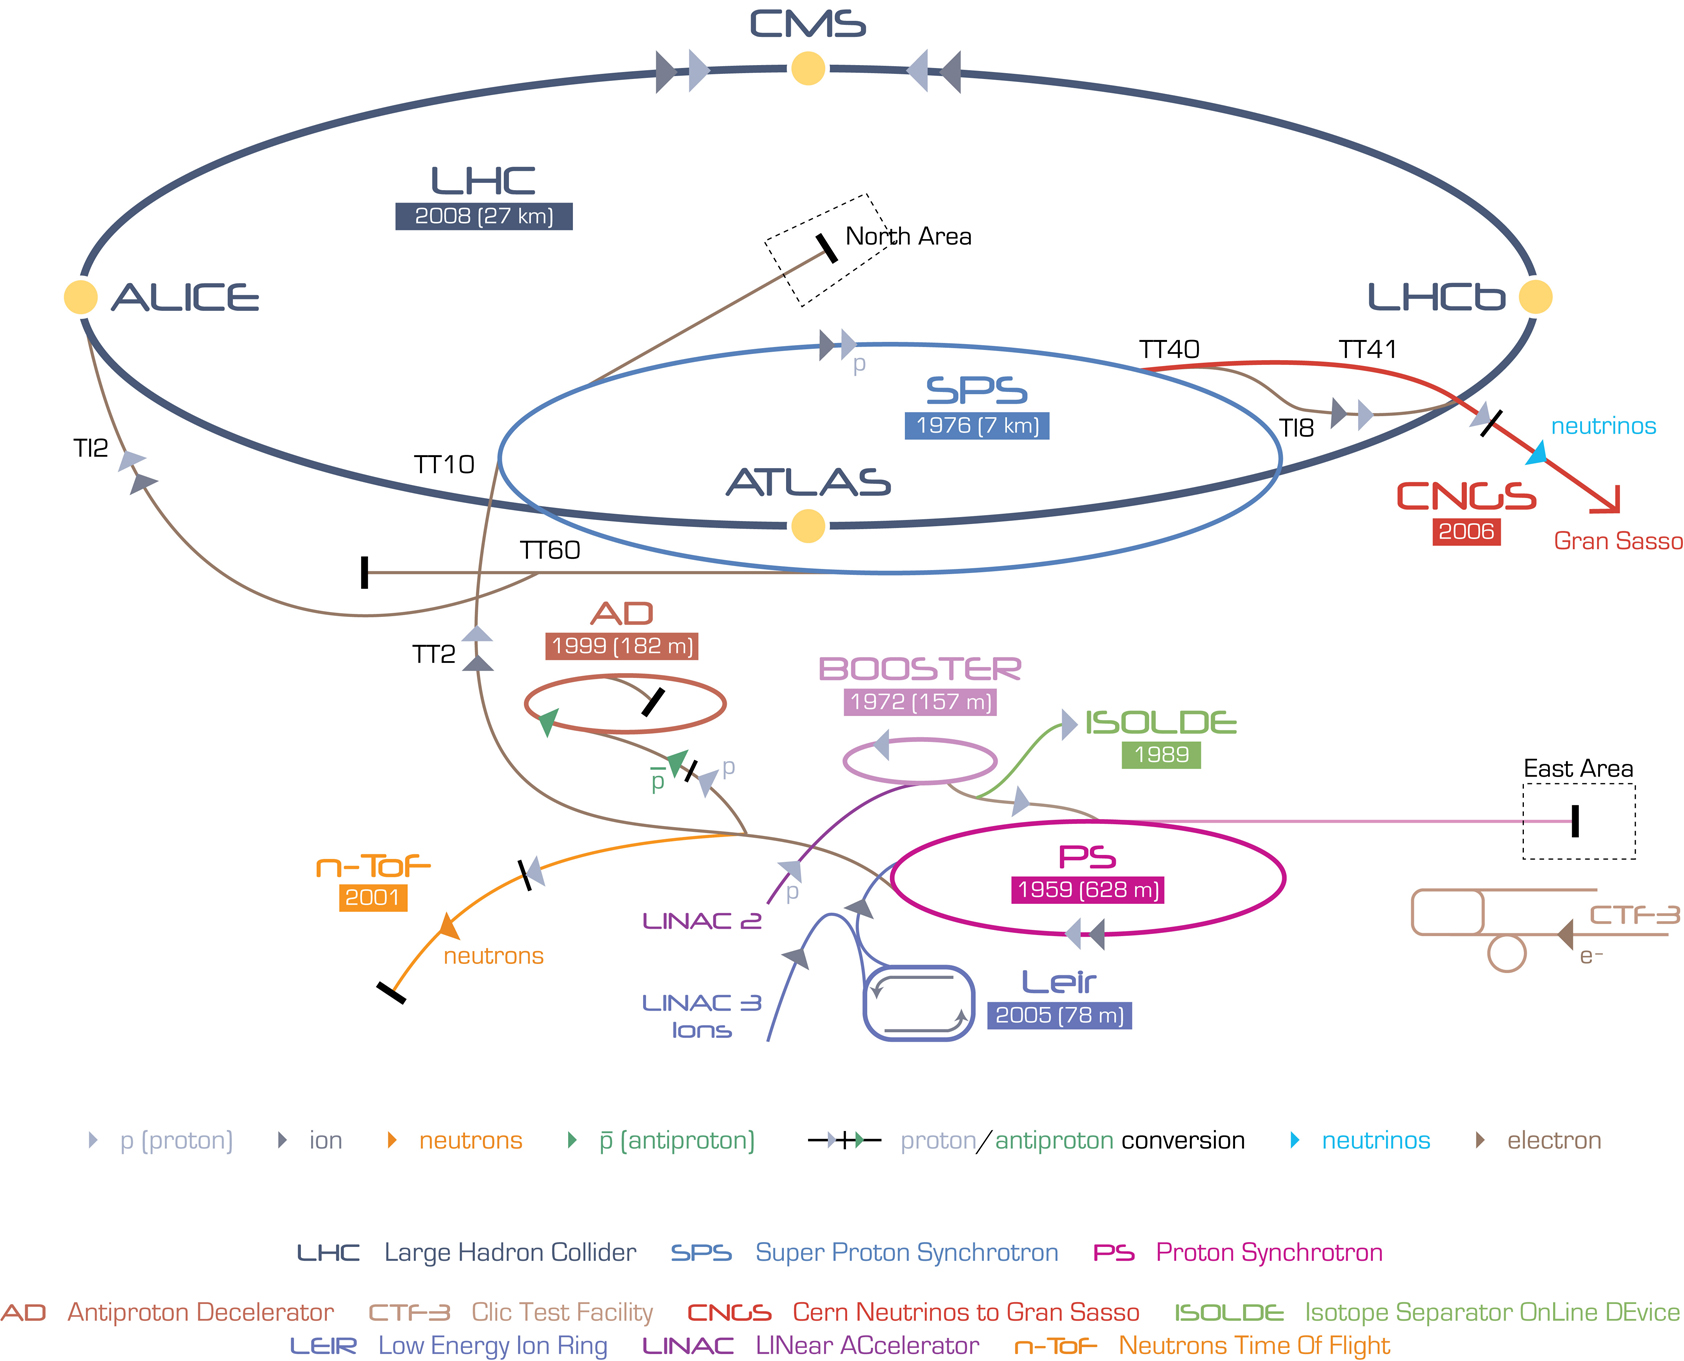
\includegraphics[width=0.74\textwidth]{Figs/machine/Cern-Accelerator-Complex.jpg}
\caption{Schematic diagram of the CERN accelerator complex, showing the various
accelerators and storage rings, ultimately feeding the Large Hadron Collider
\cite{acc_complex}.}
\label{fig:cern_acc_complex}
\end{figure}

The beams, consisting of approximately up to 1380 bunches of $\orderof(10^{11})$
protons, are brought into collision
at four points around the LHC ring within specialised detector systems, as shown
in Figure~\ref{fig:lhc_diagram}. During the
first run of the LHC, `Run I', bunches were spaced in 50~ns intervals, giving
a bunch crossing rate of 20~MHz. Collisions proceed for a number of hours, 
while collision rates are maintained by scanning the transverse beam positions, 
until such a time when proton numbers are depleted and the beam recycled so that
the fill process can be repeated.

\begin{figure}[ht!]
\centering
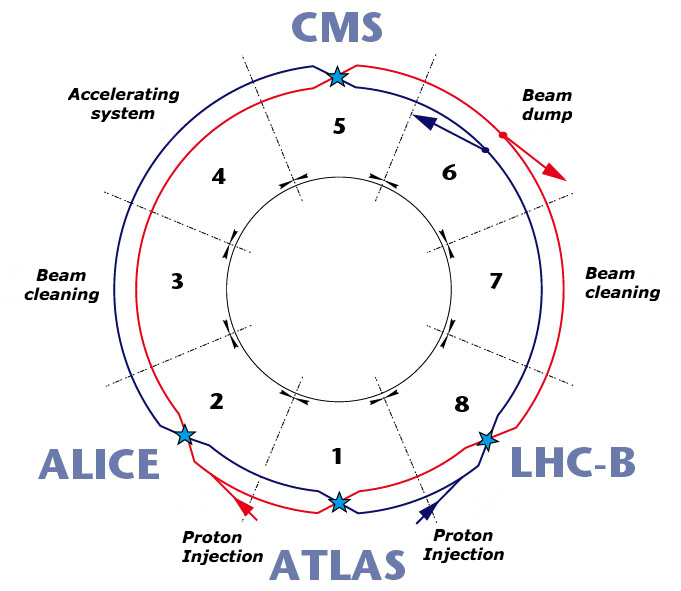
\includegraphics[width=0.6\textwidth]{Figs/machine/lhc-pho-1997-203_english.jpg}
\caption{Schematic diagram of the Large Hadron Collider, indicating the 
positions of the four collision points and their corresponding detector 
experiments \cite{Vittorio:842611}.}
\label{fig:lhc_diagram}
\end{figure}


The rate of collisions at each interaction point is described by the 
instantaneous luminosity, given by the equation:
% 
\begin{equation}
L_{inst.} = \frac{f_{orbit}n_{B}N_p^2}{A_{eff}} ,
\end{equation}
% 
where $f_{orbit}$ is the orbital frequency of bunches in the LHC, $n_B$ is the 
number of bunches in the machine, $N_p$ is the number of protons per bunch, and 
$A_{eff}$ is the effective overlap area between colliding bunches. The peak 
$L_{inst.}$ per day for CMS is shown in Figure~\ref{fig:inst_lumi_day} and the
integral over time is shown in Figure~\ref{fig:lumi_2012}, both for the full run
period through 2012.

\begin{figure}[t]
  \centering
  \begin{subfigure}[b]{0.46\textwidth}
    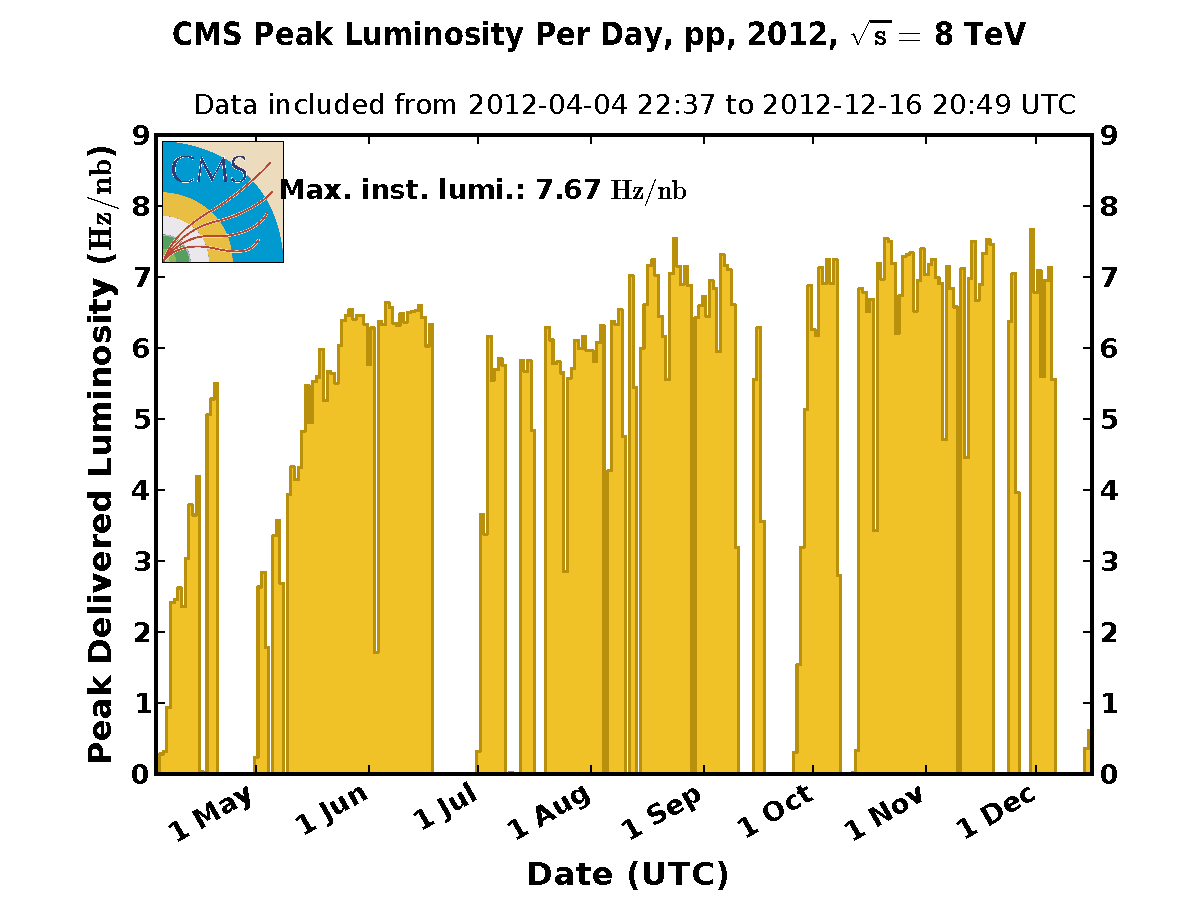
\includegraphics[width=\textwidth]{Figs/machine/peak_lumi_per_day_pp_2012.pdf}
    \caption{}
    \label{fig:inst_lumi_day}
  \end{subfigure}
  \begin{subfigure}[b]{0.46\textwidth}
    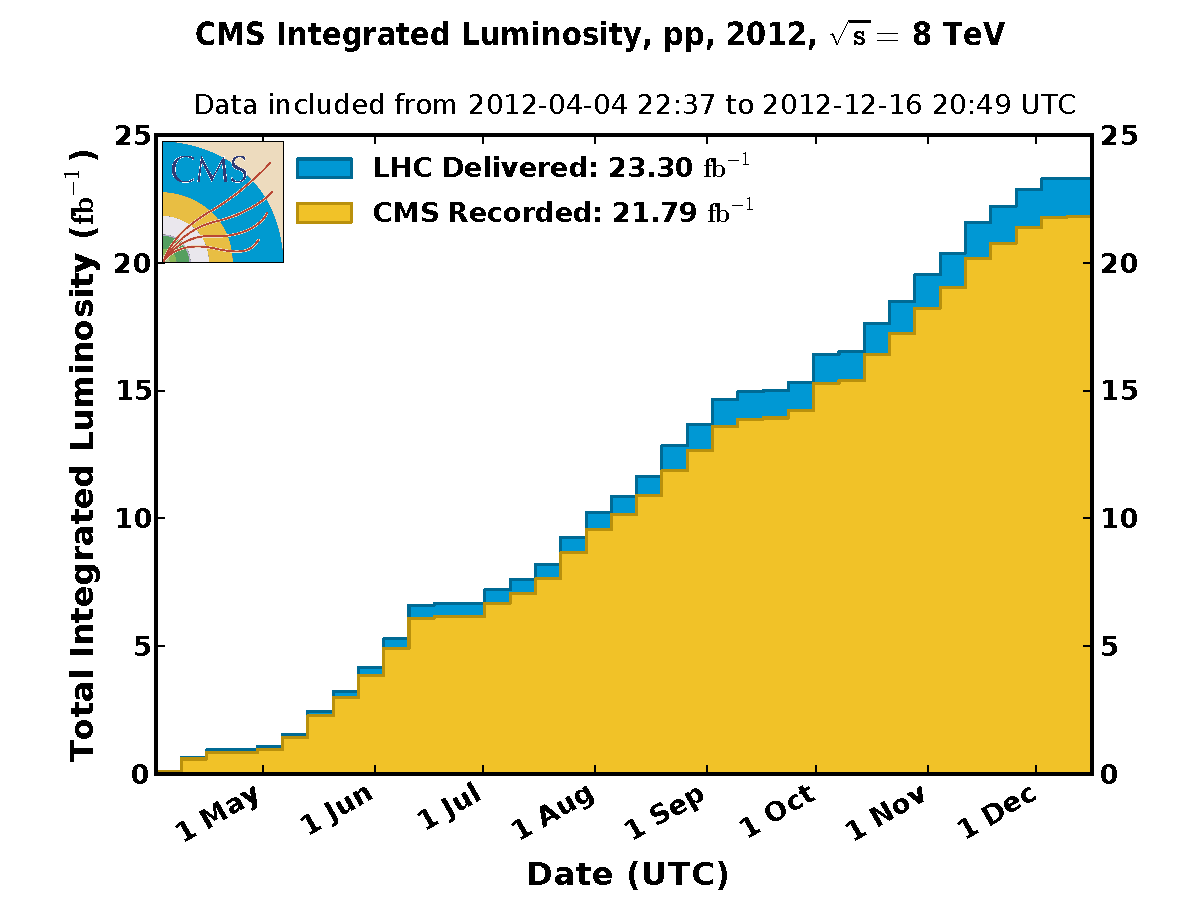
\includegraphics[width=\textwidth]{Figs/machine/int_lumi_per_week_cumulative_pp_2012.pdf}
    \caption{}
    \label{fig:int_lumi_week_cumu}
  \end{subfigure}
  \caption{The peak instantaneous luminosity for each day throughout 2012 
  (a), and the integrated luminosity delivered to and recorded at CMS (b) 
  \cite{cmslumi}.}
  \label{fig:lumi_2012}
\end{figure}

\begin{figure}
  \centering
  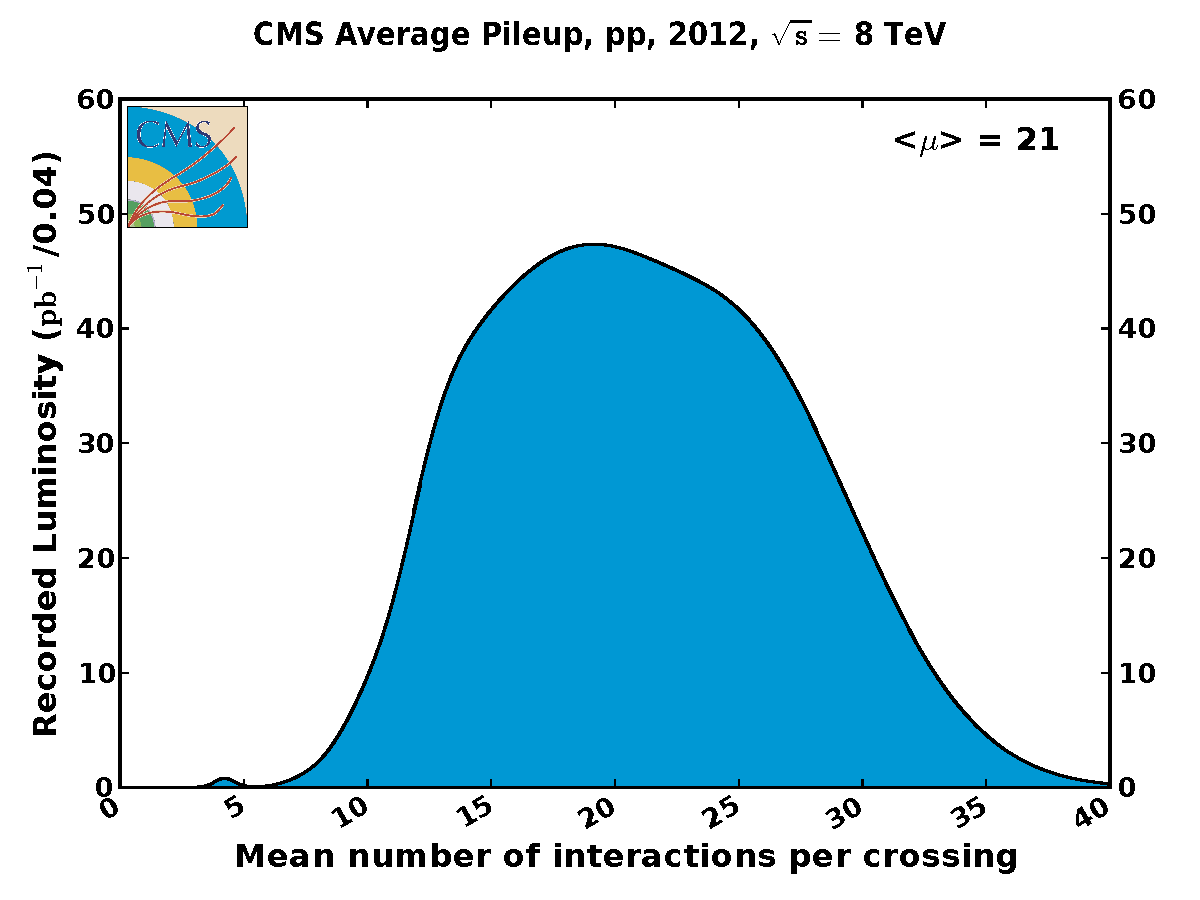
\includegraphics[width=0.6\textwidth]{Figs/machine/pileup_pp_2012.pdf}
  \caption{The average in-time pileup distribution as seen by the CMS detector
  throughout \runone~\cite{cmslumi}.}
  \label{fig:pileup_runone}
\end{figure}

Simultaneous interactions happening at the time
of each bunch crossing are referred to as in-time pile up (PU), as opposed to 
overlapping particle decays from previous bunch crossings called out-of-time 
pile up (PU). Both phenomena cause significant
experimental challenges for detector readout and event reconstruction.
The average Pileup distribution for \runone is shown in
Figure~\ref{fig:pileup_runone}.


%********************************** % Second Section  *************************************
\section{Compact Muon Solenoid}  %Section - 1.2 
\label{sec:detector_overview}

The Compact Muon Solenoid (CMS), shown in Figure~\ref{fig:cms_diagram}, is a
hermetic detector system  optimised for the study of high-\Pt objects and their
decays~\cite{CMSexperiment}.
It is designed to make accurate measurements of the positions and momenta of
physics objects such as electrons, muons, taus,
photons and jets. Owing to an almost complete 4$\pi$ solid angle coverage, CMS is 
capable of also making accurate measurements of global momentum imbalances due
to the presence of weakly interacting particles.

\begin{sidewaysfigure}
  \centering
  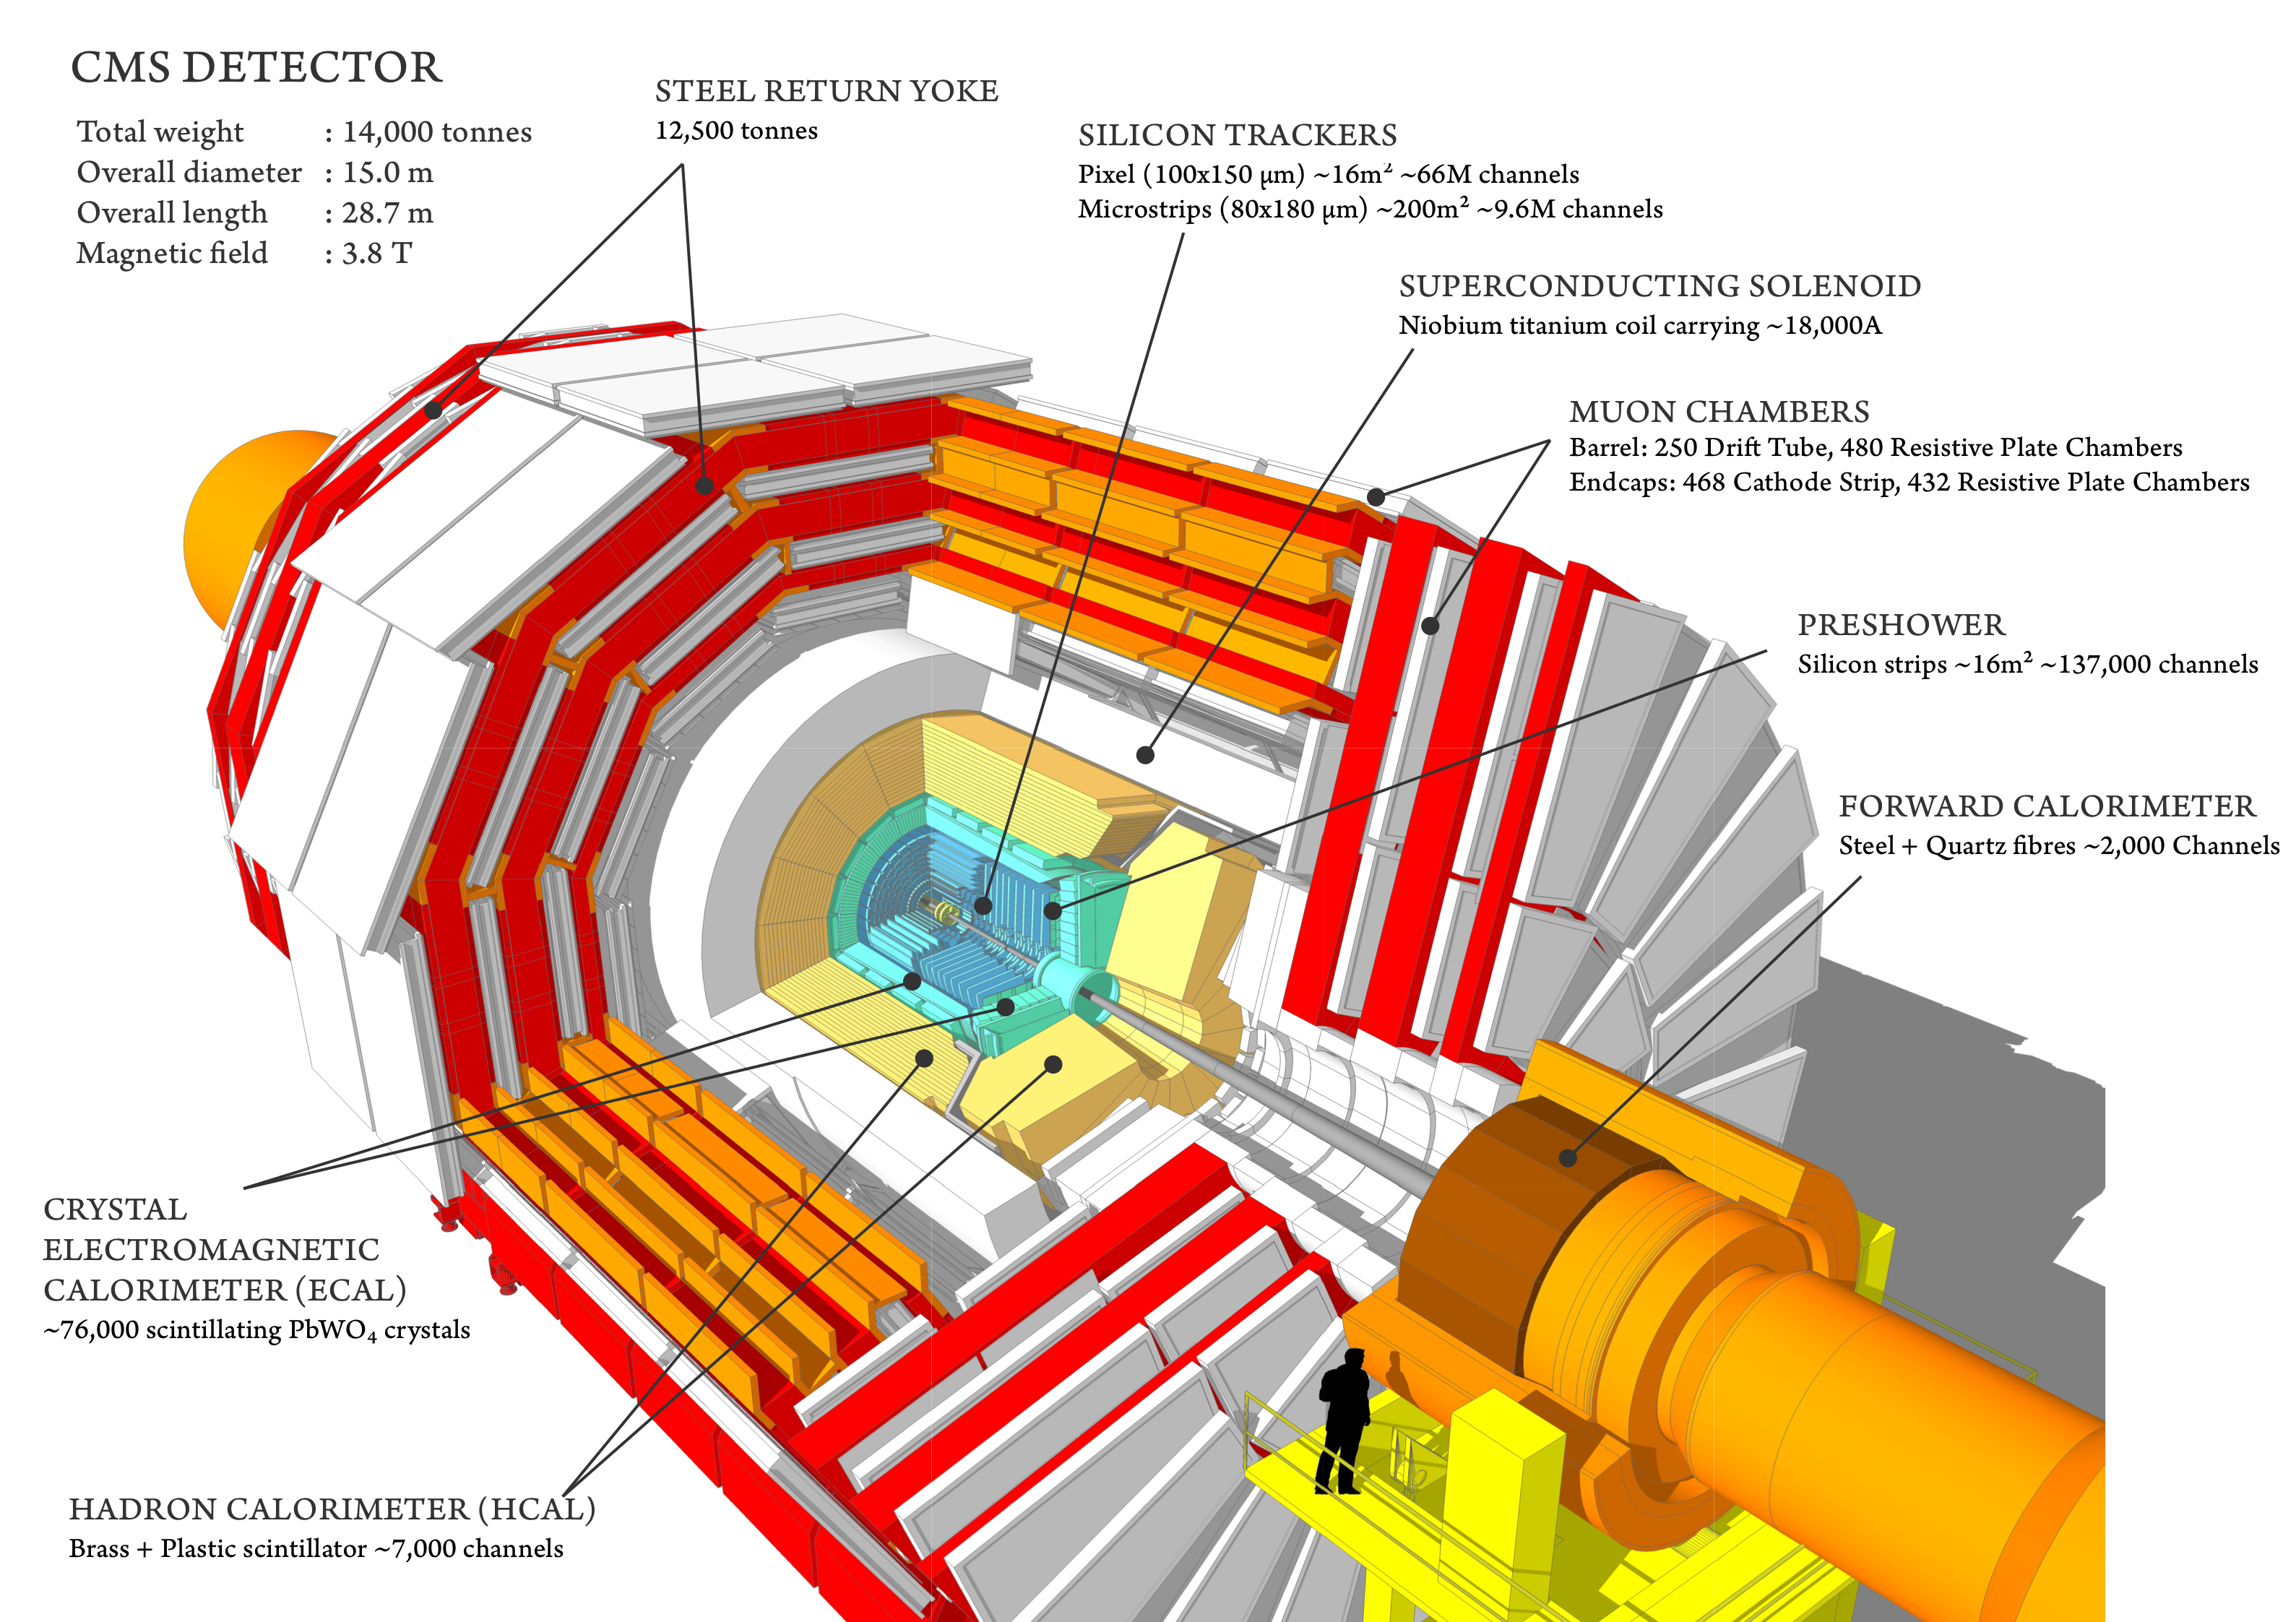
\includegraphics[width=\textwidth]{Figs/machine/cms_120918_02.png}
  \caption{Diagram of the Compact Muon Solenoid
  \cite{Sakuma:2013jqa}.}
  \label{fig:cms_diagram}
\end{sidewaysfigure}

The cylindrical detector is 28~m in length, 15~m in diameter and has a mass of 
around 14,000~tonnes. 
The z-axis is taken to be the longitudinal dimension along the beamline, the
x-axis the perpendicular direction pointing towards the centre of the LHC ring, 
and the y-axis pointing skywards, perpendicular to these forming a right-handed 
co-ordinate system. The transverse plane is taken to be the plane of the x and y
axes.

Directions relative to the CMS detector are described with the variables $\phi$,
the angular direction in the transverse plane with range $[-\pi, \pi]$, and 
`pseudo-rapidity', $\eta$, describing an angle with respect to the z-axis, defined as:
% 
\begin{equation}
\eta = - \ln \ \tan \Bigg( \frac{\theta}{2} \Bigg) ,
\end{equation}
% 
where $\theta$ is the polar angle between the particle trajectory and the beam
pipe in the y-z plane.
Differences in these two variables, namely $\Delta \phi$ and $\Delta 
\eta$, are invariant under Lorentz boosts along the beamline in the massless limit,
and so can be used to construct an angular separation between particles:
% 
\begin{equation}
\Delta R = \sqrt{ (\Delta \eta)^2 + (\Delta \phi)^2}.
\end{equation}
% 
CMS is arranged in a layered configuration of sub-detectors, structured as a 
cylindrical barrel, completed by two end-caps. The barrel contains a
super-conducting solenoid magnet capable of producing a 3.8~T magnetic field. 
Operated at 4.5~K, with a 18.5~kA current, the longitudinal field produced bends
the trajectories of charged particles allowing for precise charge and momenta 
measurements.

The following sections describe each of the detector subsystems in more detail.

\subsection{Tracker}
% - inner three layers of pixel detectors
%     - also have end-caps of pixel detectors
% - what type of pixels? what pitch? technology?
% - provide 2d information of hit positions

% - further 10 layers of silicon strip detectors
%     - n-in-p?
%     - and end-

% - this detector system provides information of not only the vertex location and 
% tracking of charged particles, but also given the massive magnet, a 
% determination of both their charge and momenta.

The silicon tracker system consists of pixel-based inner and microstrip-based
outer detectors.

The pixel detector consists of three layers of silicon pixel sensors situated 
as close as 4~cm from the beamline, capable 
of producing 2D hit information of charged particles for use in vertex 
finding with a spatial resolution of $\sim 10 \mymathhyphen 20$~\microm. The barrel section
is accompanied by two end-cap pixel detector
disks. Each sensor contains a 52 x 80 grid of individual 100~\microm x
150~\microm pixels,
mounted to a lightweight mechanical substrate along with front-end readout 
electronics.

A further 10 layers of silicon microstrip detectors are used to accurately 
reconstruct the track path of charged particles. The sensors collectively cover 
an area of over 200~$\text{m}^2$, are of p-in-n type, and range from 320~\microm
to 500~\microm in thickness and pixel pitch ranging between 80~\microm and 
205~\microm, depending on distance from the beamline. The track path can be used
to determine both the charge and momentum of charged particles, the latter with
a $\Delta \Pt/\Pt$ resolution of $\sim 1 \mymathhyphen 2 \%$ for a 100~\gev
particle.

All silicon detectors situated close to the interaction point receive
high-doses of radiation, eventually ageing due to the damage inflicted. Consequently, 
radiation hard sensor and front-end electronics materials and designs have been
selected to mitigate the effects of aging due to radiation damage.

\subsection{Electromagnetic Calorimeter}

% - ecal made of scintillating lead tungstate (PbWO4) crystals
%     - each crystal is 0.017 x 0.017 (in deltaEta x deltaPhi dimensions), and 23 
%     cm in length
%         -   corresponds to about 25 radition lengths
%         - moliere radius?
%     - super-crystal arrangement?
% - each crystal has a photodetector to determine the level of scintillation light
% produced
%     - avalanche photo-diodes in the barrel, and vacuum photo-triodes in the 
%     endcap region
%     - radiation hardness?
%     - what material?

% - this detector system provides energy and spatial information of
% electromagnetically showering particles.

The Electromagnetic Calorimeter (ECAL) system provides accurate measurements of 
energy deposits and the identification of electromagnetically interacting 
particles, and can also produce spatial measurements when used in conjunction 
with data from the tracker system. The detector consists of scintillating
lead-tungstate
($\text{PbWO}_4$) crystals, each of dimension 0.017 x 0.017 ($\Delta \eta \times
\Delta \phi$) and 23~cm in length, corresponding to approximately 26 radiation
lengths
and providing a Moli\`{e}re radius of 2.2~cm. In both the barrel and the
end-cap regions, individual crystals are clustered into super-towers, to match
with towers in the trigger system (the calorimeter trigger system is described
later in Section~\ref{sec:detector_trigger}).

Scintillation light produced in each crystal is collected by either
avalanche photo-diodes in the barrel or vacuum photo-triodes in the
endcap. The detectors are required to be both radiation hard and capable of
operating within the strong magnetic field environment of CMS.

The ECAL system is measured as having a $\Delta E/E$ resolution for a 100~\gev
particle of $\sim 0.5\%$, exceeding its technical design requirements.

\subsection{Hadronic Calorimeter}

% - alternating layers of brass absorber and plastic scintillator
% - scintillators are sectioned into towers, 0.087x0.087 in barrel and 0.17x0.17 
% in the endcaps (double check this isn't just my interpretation of ted's eta 
% numbers)
% - light produced in the scintillator layers is transmitted via wavelength 
% shifting fibres to a hybrid photo-diode for detection

The Hadronic Calorimeter (HCAL) system measures the energy of hadronic showers 
originating from single-quarks and gluons (i.e. jets). It is constructed from
layers of alternating brass absorber and plastic scintillator, of which there
are 17 in the barrel and 19 in the endcaps. The latter are spatially
divided into towers measuring 0.087 x 0.087 in the barrel and end-caps. Hadronic
particle showers deposit energy as scintillation light in the plastic layers,
which is transmitted via wavelength shifting fibres to be measured in hybrid
photo-diodes. The energy resolution of the HCAL system is calculated with
respect to $\pi$-meson energy reconstruction, and is measured to be
$\sim 90\%/\sqrt{E}~\text{\gev}^{-0.5}$ in the barrel,
and $\sim 100\%/\sqrt{E}~\text{\gev}^{-0.5}$ in the endcap.

\subsection{Muon Systems}

% - comprised of three different gaseous detector technologies, each with 
% different coverages in eta
% - drift tubes (DT)
%   - traditional technology, optimised for low occupancy
%   - central: eta < 1.2
% - cathode strip chambers (CSC)
%   - designed for high magnetic field and neutron backgrounds
%   - forward: 0.9 < eta < 2.4
% - resistive plate chambers (RPC)
%   - designed for high magnetic field and neutron backgrounds
%   - forward and central eta < 2.1

The muon system provides identification and precision measurements of
muon position and momenta. Energy deposits in the muon systems can be combined
with corresponding information from the tracker to improve momentum resolution
significantly. The system is designed to have a momentum resolution,
$\Delta \Pt/\Pt$, of
$\sim10\%$ on its own, and $\sim2\%$ when combined with tracker information,
both measured for muons with \Pt < 100~\gev.

\begin{figure}[ht!]
\centering
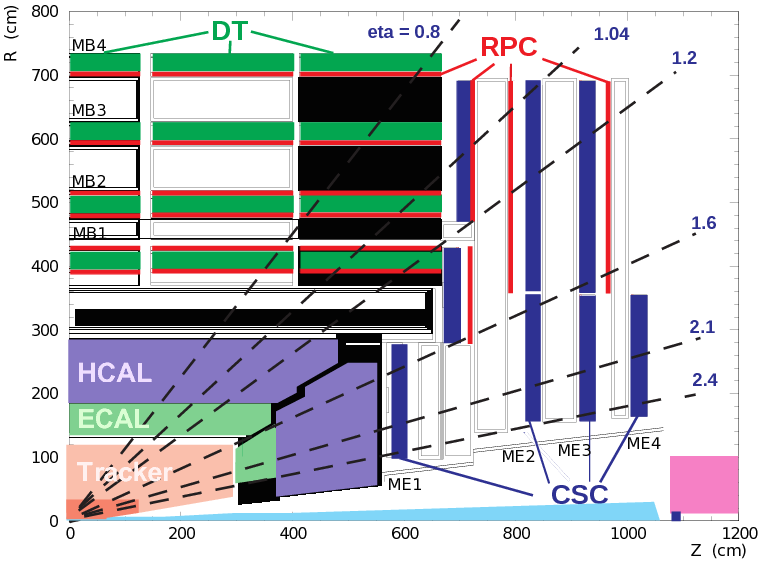
\includegraphics[width=0.6\textwidth]{Figs/machine/pictures_MuonSys-mod3.png}
\caption{Cross section of the CMS detector in the $y\mymathhyphen z$ plane,
showing the three muon systems (DT, RPC and CSC) as well as other interior sub-detector systems~\cite{Bayatian:922757}.}
\label{fig:muon_system_diagram}
\end{figure}

Muons are detected in the outer layers of CMS, with the muon system 
comprised of three different gaseous detector technologies each with different 
pseudo-rapidity coverage, as shown in Figure~\ref{fig:muon_system_diagram}. The
central barrel region, $|\eta|<1.2$, is equipped with 
Drift Tube (DT) detectors - a traditional detector technology, optimised for low
-occupancy measurements. Cathode Strip Chambers (CSC) cover the forward region,
$0.9 < |\eta| < 2.4$, and dual-layered Resistive Plate Chambers (RPC) cover
$|\eta| < 2.1$ - both CSC and RPC detectors being optimised for operation in 
the presence of both high magnetic field and neutron background environments.


\subsection{Trigger}
\label{sec:detector_trigger}
Events of interest are selected using a dedicated triggering system~\cite{tridasTDR},
divided into two distinct stages: the hardware-based Level-1 Trigger (L1) and
the software-based High-Level Trigger (HLT).

\subsubsection{Level-1 Trigger}
% - L1 system is hardware based running at a rate of 40 MHz
% - runs on coarse trigger primitive objects, constructed from raw energy deposits
% in the calorimeter and muon systems independently
%     - takes regional information from both the calorimeter and muon systems 
%     independently.
%     - combines regional data in the GCT/GMT
%     - feeds combined objects (from across entire detector) into the GT, where a 
%     L1 accept is made or not.
% \emph{can talk in more detail here about the calorimeter trigger path and the 
% GCT's job}
% - has approximately 3microsecs per events
% - objects considered at L1 are electrons, muons, jets (central and forward) and 
% energy sums (ETT, MET, HTT, MHT)
% - L1Accept is made dependent on the objects within an event meeting 1 of 127 (
% check!) simple threshold and multiplicity based requirements.
% - maximum available output bandwidth of the L1 system is 100 kHz, although the 
% output rate is kept lower than this to allow for stochastic fluctuations

The L1 system consists of a staged, modular design of custom built hardware 
electronics subsystems, as shown in Figure~\ref{fig:l1_diagram}. 
The L1 trigger reconstructs energy deposits in the calorimeter and muon systems
into coarse `trigger-primitive' physics objects.
Regional information is gathered by separate modules 
before being combined in the Global Calorimeter Trigger (GCT) and Global Muon 
Trigger (GMT) systems, where physics objects are sorted according to energy. 
Finally, event objects are passed on to the Global Trigger (GT) where a 
`Level-1 Accept' (L1A) signal is issued or not, dependent on the event meeting 
one of up to 128 simple object threshold and multiplicity based requirements.

\begin{figure}[ht!]
  \centering
  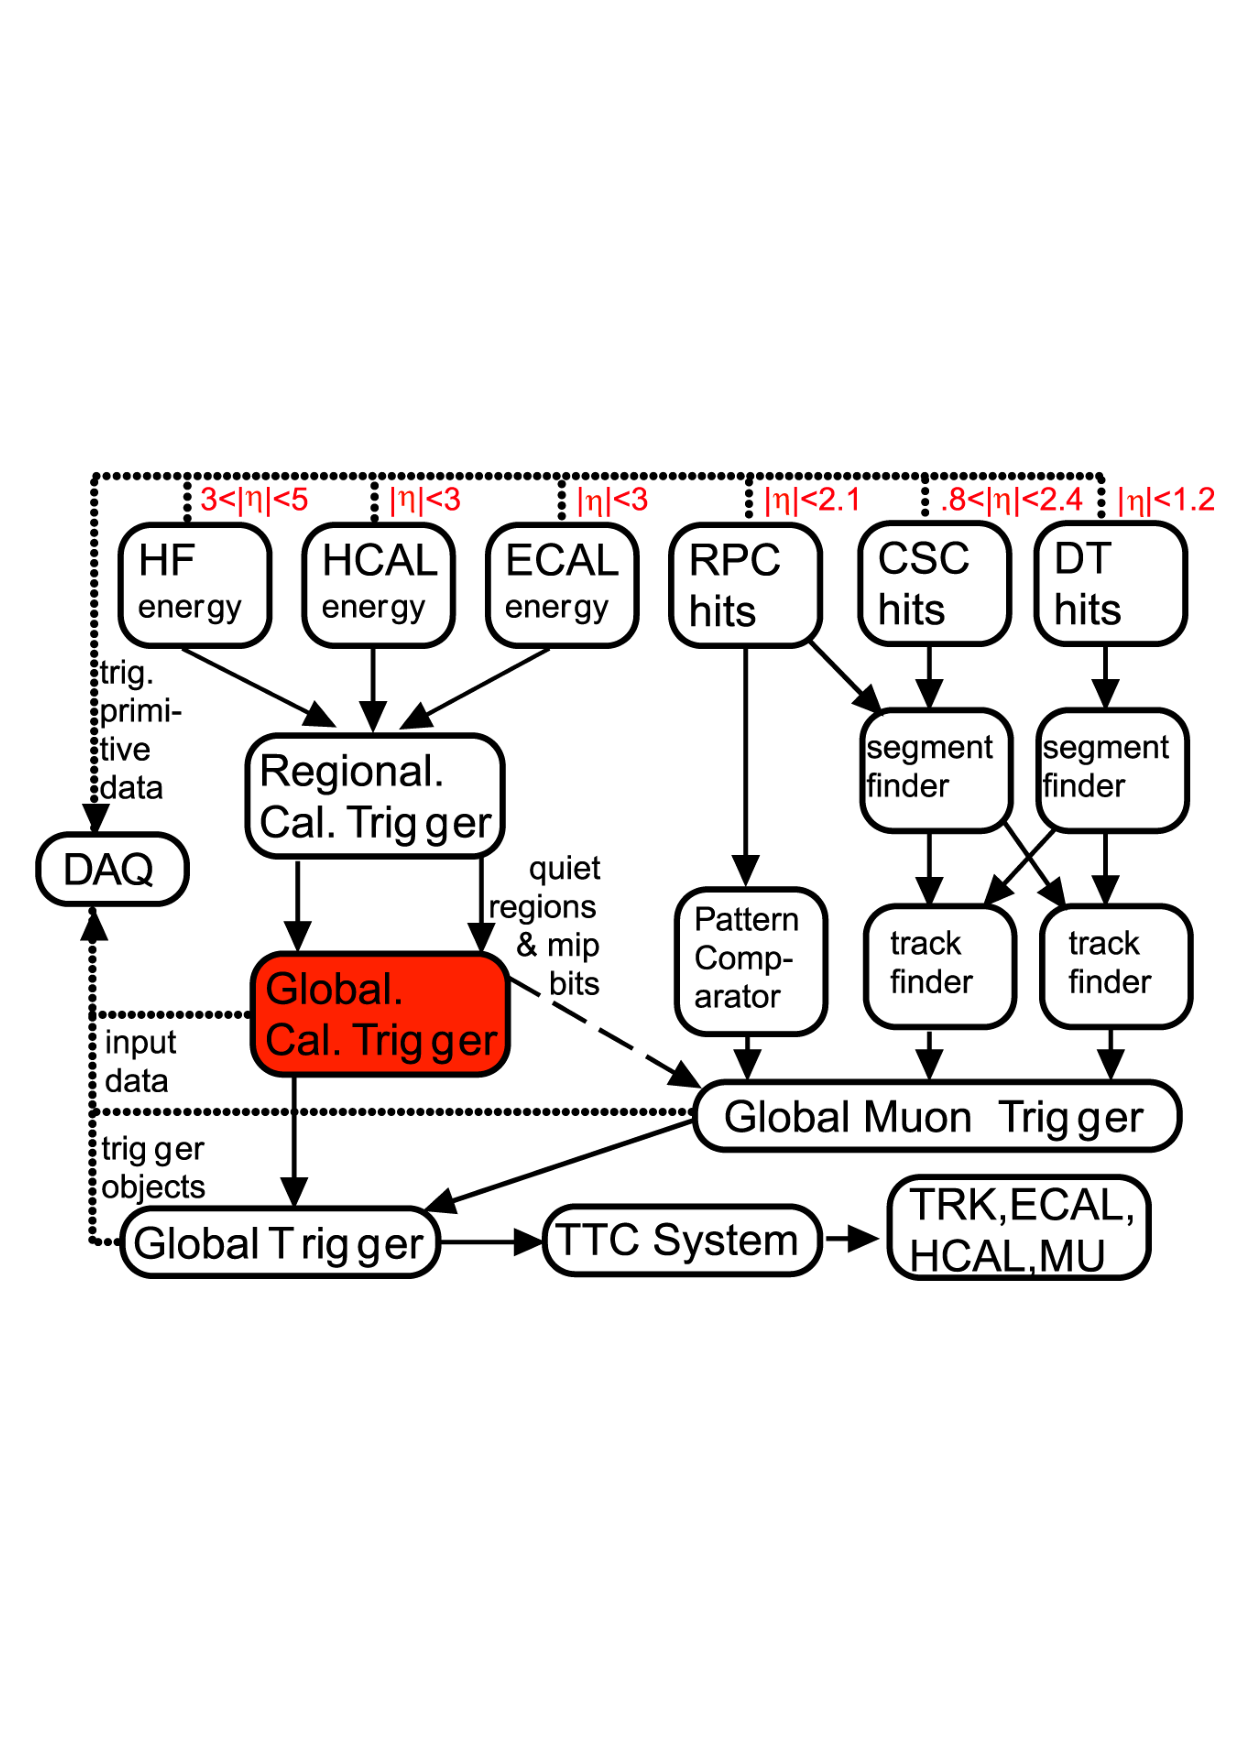
\includegraphics[width = 0.55\textwidth]{Figs/machine/L1_diagram.pdf}
  \caption{Schematic overview of the Level-1 hardware trigger system of CMS. $
  \eta$ coverage is shown in red text and the data-flow indicated by arrow 
  direction~\cite{tridasTDR}.}
  \label{fig:l1_diagram}
\end{figure}

The L1 system is required to run at 40~MHz, equal to the maximal bunch-crossing
rate within CMS, with a L1A decision required within a latency of 3 $\mu \text{s}$. The
maximum available output bandwidth of the L1 system is 100~kHz, but typically is
maintained at a lower value to allow for stochastic fluctuations in rate.

\subsubsection{High-level Trigger}
% - Following a L1A signal, candidate events are optically transmitted to the high
% level trigger, consisting of a large computer farm of the off the shelf server 
% PCs
% - events are reconstructed/built in more detail
% - passed on to a suite of analyst-designed software triggers which can 
% reconstruct more advanced objects and event variables, such as alphaT (as 
% described later in chapter BLAH) - has approximately 50ms per event
% - HLT reduces rate to around 300 events per second

Following a L1A signal, candidate events are optically transmitted to the HLT 
system, consisting of a large computer farm of server 
PCs. Due to the increase in available processing time of up to 50 ms, events can
be reconstructed in greater detail allowing for a closer emulation of offline 
reconstruction techniques. Complex analyst-designed trigger rules are used, 
which can employ more sophisticated event-level variables such as \alphat
(described in detail later in Chapter~\ref{ch:analysis}).

The HLT reduces the event rate further by around two orders of magnitude,
producing an output event rate of up to 1~kHz. Events passing the HLT are
transmitted to the Grid computing system~\cite{Eck:840543} for full offline
reconstruction.
